\documentclass{beamer}
\usetheme{CambridgeUS}

%\setbeamertemplate{caption}[numbered]{}

\usepackage{enumitem}
\usepackage{tfrupee}
\usepackage{amsmath}
\usepackage{amssymb}
\usepackage{gensymb}
\usepackage{graphicx}
\usepackage{txfonts}

\def\inputGnumericTable{}

\usepackage[latin1]{inputenc}                                 
\usepackage{color}                                            
\usepackage{array}                                            
\usepackage{longtable}                                        
\usepackage{calc}                                             
\usepackage{multirow}                                         
\usepackage{hhline}                                           
\usepackage{ifthen}
\usepackage{caption} 
\captionsetup[table]{skip=3pt}  
\providecommand{\pr}[1]{\ensuremath{\Pr\left(#1\right)}}
\providecommand{\cbrak}[1]{\ensuremath{\left\{#1\right\}}}
\renewcommand{\thefigure}{\arabic{table}}
\renewcommand{\thetable}{\arabic{table}}                                     
                               
\title{AI1110 \\ Assignment 8}
\author{Sai Pradeep \\ AI21BTECH11013}
\date{\today}


\begin{document}
	% The title page
	\begin{frame}
		\titlepage
	\end{frame}
	
	% The table of contents
	\begin{frame}{Outline}
    		\tableofcontents
	\end{frame}
	
	% The question
	\section{Question}
	\begin{frame}{Exercise 6.42}
	Q: x and y are independent random variables with geometric p.m.f.
	$$\pr{x=k}=p q^k$$ k= 0,1,2,... $$\pr{y=m}=p q^m $$ m= 0,1,2,...
 Find the p.m.f. of
\begin{enumerate}[label=(\alph*)]
 \item x+y
 \item x-y
 \end{enumerate}	
	\end{frame}

	% The solution
	\section{Solution}
	\begin{frame}{Solution}
    X,Y are independent geometric random variables.Thus
    \begin{align}
    \pr{X=k,Y=m} &= \pr{X=k} \times \pr{Y=m}\\
    &=(p \times q^k) \times (p \times q^m)\\
    &=p^2 \times q^(k+2)
    \end{align}
\begin{enumerate}[label=(\alph*)]
     \item  Let $$Z=X+Y$$
     \begin{align}
     \pr{Z=n}&=\pr{X+Y=n}\\
     &=\sum\limits_{k=0}^n \pr{X=k,Y=n-k}\\ 
     &=\sum\limits_{k=0}^n \pr{X=k} \times \pr{Y=n-k}
     \end{align}
    \end{enumerate}
    \end{frame}
    
	\begin{frame}{Computation}
	    \begin{align}
	       \pr{Z=n}&=\sum\limits_{k}^n (p \times q^k) \times (p \times q^(n-k))\\
         &=(n+1)p^2 q^n  n=0,1,2,3,.....
	    \end{align}
\begin{enumerate}[label=(\alph*)]
  	    
    Let W=X-Y\\
    \end{enumerate}
	 Case-1:
	    \begin{align}
	     W \geq 0 \implies X \geq Y
	     \end{align}
	 Thus for $ m \geq 0$
	 \begin{align}
	 \pr{W=m} &= \pr{X-Y=m}\\
     &=\sum\limits_{k=0}^\infty \pr{X=m+k,Y=k}\\
     &=\sum\limits_{k=0}^\infty \pr{X=m+k,Y=k}\\
     \end{align}
     \end{frame}
     
     \begin{frame}{Computation}
     \begin{align}
     &=\sum\limits_{k=0}^\infty \pr{X=m+k}{Y=k}\\
     &=\sum\limits_{k=0}^\infty (p q^m+k) \times (p q^k)\\
     &=p^2 q^m \sum\limits_{k=0}^\infty q^2k\\
     &=p^2 q^m \times (1+q^2 + q^4 +....)\\
     &=\dfrac{p^2 q^m}{1-q^2}
     \end{align}
      Since $p=1-q$ and $1-q^2=(1-q) \times (1+q)$
	
	 \end{frame}
	 
	 \begin{frame}{Computation}
	 
	 \begin{align}
	 \label{eq:eq1}
	 \pr{W=m} &=\dfrac{p^2 q^m}{1+q}  m=0,1,2,...
	 \end{align}
      Let $W=X-Y$\\
      Case -2:
      \begin{align}
	     W < 0\\
	 \implies X < Y
	  \end{align}
	 Thus for $m < 0$\\
	 \begin{align}
	 \pr{W=m} &= \pr{X-Y=m}\\
     &=\sum\limits_{k=0}^\infty \pr{X=k,Y=k-m}
     \end{align}
     \end{frame}
     
     \begin{frame}{Computation}
     \begin{align}
     &=\sum\limits_{k=0}^\infty \pr{X=k,Y=k-m}\\
     &=\sum\limits_{k=0}^\infty \pr{X=k}{Y=k-m}\\
     &=\sum\limits_{k=0}^\infty (p q^k) \times (p q^{k-m})\\
     &=p^2 q^{-m} \sum\limits_{k=0}^\infty q^2k\\
     &=p^2 q^{-m} \times (1+q^2 + q^4 +....)\\
     &=\dfrac{p^2 q^{-m}}{1-q^2} 
     \end{align}
    
     \end{frame}
     
     \begin{frame}{Conclusion}
      Since $p=1-q$ and $1-q^2=(1-q) \times (1+q)$
	 \begin{align}
	 \label{eq:eq2}
	 \pr{W=m}&=\dfrac{p^2 q^{-m}}{1+q} m=-1,-2,...
	 \end{align}
	     Hence from equations \eqref{eq:eq1} and \eqref{eq:eq2} ,We can write that
	     \begin{align}
	   \pr{W=m}&=\dfrac{p q^{\mid x \mid}}{1+q} m=0,\pm 1,\pm 2,....       
	     \end{align}
	 \end{frame} 
	 \section{Graph}
\begin{frame}{Output graph for p=0.7}
    \begin{figure}[!ht]
		\centering
		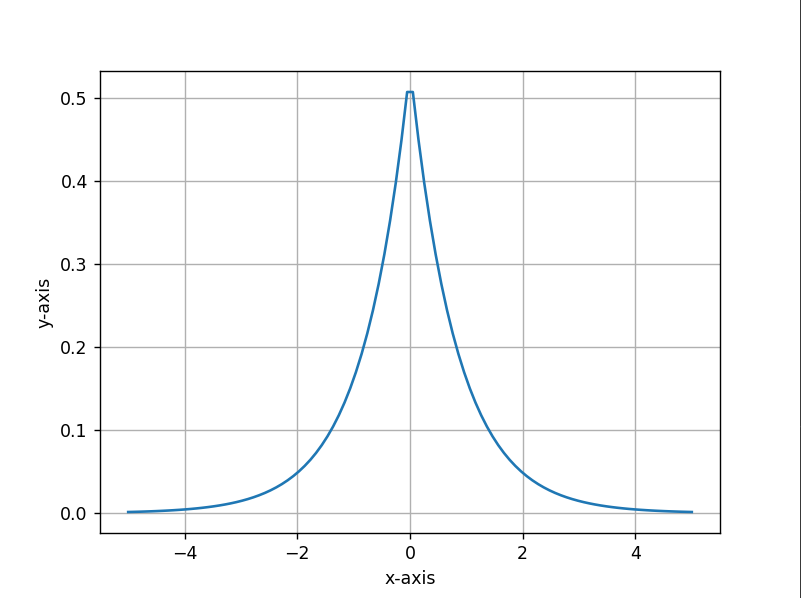
\includegraphics[width=\textwidth,height=6.5cm,keepaspectratio]{figures/fig1.png}
		\caption{fig 1}
		\label{fig1}
	\end{figure}
\end{frame}
	 
\end{document}
